\documentclass{article}
\usepackage{amsmath}
\usepackage{graphicx}
\usepackage{needspace}
\usepackage{geometry}
\usepackage{amssymb}
\usepackage{hyperref}
\usepackage{listings}

% set href color to blue with underline
\hypersetup{
    colorlinks=true,
    linkcolor=black, 
    filecolor=magenta,      
    urlcolor=cyan,
    pdftitle={Projet GNN - Rapport},
    pdfpagemode=FullScreen,
}

\title{Projet BIML - Rapport}
\author{Axel COLMANT}
\date{\today}

% Additional information
\newcommand{\matiere}{Bio-Inspired Machine Learning}
\newcommand{\professeur}{Rémy Cazabet}

% Change geometry of the page
\geometry{
    a4paper,
    left=30mm,
    right=30mm,
    top=30mm,
    bottom=30mm
}
\pagestyle{plain}

\begin{document}

\maketitle

\begin{center}
    \textbf{Matière:} \matiere \\
    \textbf{Professeur:} \professeur
\end{center}

\vspace{1cm}

\tableofcontents
\clearpage

\section{Introduction}

Ce projet se penche sur la possibilité de classifier les aéroports par pays à partir d'un graphe non orienté où les sommets sont les aéroports et les arêtes les routes aériennes. Pour cela nous utiliserons tout au long des expérimentations un modèle GCN (Graph Convolutional Network) qui est un modèle de deep learning spécialisé pour les graphes.\\
Nous nous intéressons particulièrement à l'influence de différents facteurs sur la performance de la classification, tels que la position géographique des aéroports, la population des villes desservies et la structure du graphe de connexions aériennes. Notre hypothèse principale est que l'ajout d'informations démographiques, en complément des données géographiques, améliorera la précision de la classification.  Pour valider cette hypothèse, nous allons réaliser une série d'expérimentations en utilisant différentes configurations d'attributs et de structures de graphe,  et en évaluant les performances de différents algorithmes de classification.\\

Pour visualiser les résultats, nous utiliserons un affichage spaciale que nous comparerons à la carte suivante représentant les aéroports classifiés par pays.\\

\begin{figure}[h!]
    \centering
    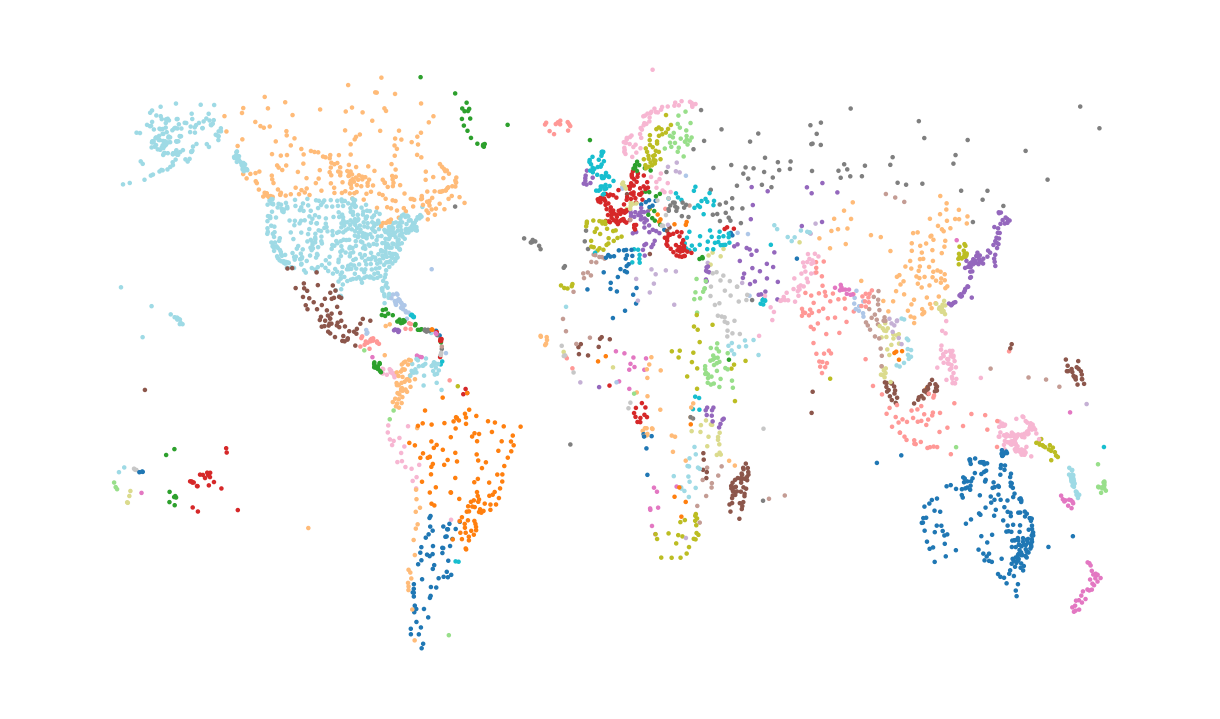
\includegraphics[width=\textwidth]{content/img/map-airports-goal.png}
    \caption{Carte des aéroports classifiés par pays (objectif)}
    \label{fig:map}
\end{figure}

\section{Données}
Les données utilisées pour ce projet proviennent du fichier \href{http://cazabetremy.fr/Teaching/IAbioInspire/airportsAndCoordAndPop.graphml}{airportsAndCoordAndPop.graphml} fourni par le professeur, Remy Cazabet

\subsection{Description des données}

Ce fichier est un graphe non orienté où les sommets sont les aéroports et les arêtes les routes aériennes. Chaque sommet est caractérisé par les attributs suivants:
\begin{itemize}
    \item \textbf{country}: le nom du pays de l'aéroport (string)
    \item \textbf{city\_name}: la nom de la ville de l'aéroport (string)
    \item \textbf{lat}: la latitude de l'aéroport (float)
    \item \textbf{lon}: la longitude de l'aéroport (float)
    \item \textbf{population}: la population de la ville de l'aéroport (int)
\end{itemize}

\subsection{Prétraitement des données}
Avant d'appliquer les algorithmes de classification, nous avons effectué un pré-traitement des données afin de les adapter à notre modèle GCN. 

\begin{itemize}
    \item {
        \textbf{Filtering}: J'ai filtré les données pour ne conserver que les aéroports des pays pour lesquels nous avons un grand nombre d'exemples. Cela nous permettra d'avoir un jeu de données plus équilibré et éviter les biais dus à un faible nombre d'exemples pour certains pays.\\
        \textit{Pour mes tests j'ai principalement utilsié ces trois valeurs: 10, 50 et 100. Qui donne respectivement 67, 12 et 4 pays différents.}
    }
    \item {
        \textbf{Selection}: J'ai sélectionné les attributs d'entrée et de sortie du modèle. Les attributs d'entrée sont \textit{lat}, \textit{lon} et \textit{population}, tandis que l'attribut de sortie est \textit{country}.
    }
    \item {
        \textbf{Encoding}: J'ai encodé les attributs catégoriels \textit{country} et \textit{city\_name} en utilisant un \textit{LabelEncoder} de la librairie \textit{scikit-learn}. Cela permet de transformer les noms de pays et de villes en entiers, ce qui est nécessaire pour les utiliser dans un modèle de machine learning.
    }
    \item {
        \textbf{Normalization}: J'ai normalisé les attributs \textit{lat}, \textit{lon} et \textit{population} en utilisant un \textit{StandardScaler} de la librairie \textit{scikit-learn}. Cela permet de mettre à la même échelle les différentes caractéristiques des données, ce qui est important pour l'entraînement de modèles de machine learning.
    }
    \item {
        \textbf{Splitting}: J'ai divisé les données en ensembles d'entraînement, de validation et de test (80\%, 10\%, 10\%). Cela permet d'évaluer la performance du modèle sur des données qu'il n'a pas vues pendant l'entraînement.
    }
    \item {
        \textbf{Autres}: J'ai effectué d'autres types de prétraitement spécifiques à certains tests que j'ai réalisés, tels que la création de graphes de connexions aériennes pondérés par la distance géographique entre les aéroports.
    }
\end{itemize}

Ce pré-traitement nous permet d'obtenir des données structurées sous forme de graphes,  prêtes à être utilisées par notre modèle GCN.  En variant les attributs et la structure du graphe,  nous pourrons analyser l'influence de ces facteurs sur la performance de la classification des aéroports par pays.
\section{Methode de classification}
Pour cette étude, j'ai choisi d'utiliser un modèle de Graph Convolutional Network (GCN) pour la classification des aéroports. 

\subsection{Graphe Convolutional Network (GCN)} 
Les GCN sont des réseaux de neurones spécifiquement conçus pour traiter des données structurées sous forme de graphes,  ce qui les rend particulièrement adaptés à notre problématique.  
Ils permettent d'apprendre des représentations vectorielles des nœuds (dans notre cas, les aéroports) en tenant compte à la fois des informations propres à chaque nœud (attributs) et de la structure du graphe (connexions avec les autres nœuds).\\
Ils sera donc intéressant d'interpréter les résultats obtenus pour comprendre comment les diffétents attributs et la structure du graphe influent sur sa capacité à classifier les aéroports par pays.\\
\\
Le modèle GCN que nous avons utilisé est composé de trois couches de convolution, chacune suivie d'une fonction d'activation ReLU. La dernière couche est suivie d'une fonction d'activation softmax
pour obtenir une distribution de probabilité sur les pays.\\
% Code embelling
\begin{lstlisting}[language=Python]
class GCN(nn.Module):
    def __init__(self, dim_in, dim_h, dim_out):
        super(GCN, self).__init__()
        self.conv1 = gnn.GCNConv(dim_in, dim_h)
        self.conv2 = gnn.GCNConv(dim_h, dim_h)
        self.conv3 = gnn.GCNConv(dim_h, dim_out)
        
        
    def forward(self, x, edge_index, edge_weight):
        x = F.relu(self.conv1(x, edge_index, edge_weight))
        x = F.relu(self.conv2(x, edge_index, edge_weight))
        x = self.conv3(x, edge_index, edge_weight)
        return  F.log_softmax(x, dim=1)
\end{lstlisting}


\subsection{Métriques d'évaluation}
Pour évaluer la performance de notre modèle, nous avons utilisé deux métriques d'évaluation: la précision. 
La précision est le nombre de prédictions correctes divisé par le nombre total de prédictions. Elle permet de mesurer la capacité du modèle à classifier correctement les aéroports par pays.\\




\section{Experimentation et résultats}

\subsection{Configurations testées}

Afin d'évaluer l'influence des différents facteurs sur la performance de la
classification des aéroports par pays, j'ai réalisé une série
d'expérimentations en faisant varier les paramètres suivants :

\begin{enumerate}
    \item {
          \textbf{Nombre d'aéroports par pays} : Permet de tester les performances du modèle en faisant varier le nombre d'aéroports par pays. Voici les configurations suivantes : 10, 20, 30, 40, 50, 60, 70, 80, 90 et 100 aéroports par pays.
          }
    \item {
          \textbf{Influence des features} : J'ai testé les performances du modèle en faisant varier les features utilisées pour la classification. Nous avons testé les configurations suivantes :[latitude, longitude]; [latitude, longitude, population]; [population].\\
          \textit{Note} : J'ai également fait varier le nombre d'aéroports par pays pour chaque configuration de features (10, 50, 100).
          }
    \item {
          \textbf{Pondération des liens} : J'ai testé sur différentes configurations de nombre d'aéroports par pays (10, 50, 100) l'influence de la pondération des liens sur la performance du modèle. Et comparé les résultats obtenus avec et sans pondération des liens.
          }
    \item {
          \textbf{Structure du graphe} : J'ai terminé par tester les performances du modèle en faisant varier la structure du graphe (Fully-connected, Country-based).
          }
\end{enumerate}

\subsection{Analyse des résultats}

Dans cette section, je vais analyser les résultats obtenus. Je m'appuierai
principalement sur les données de précision et d'erreur pour chaque
configuration testée.\\

\needspace{10\baselineskip}
\subsubsection{Nombre d'aéroports par pays}
Mon objectif ici à été de comprendre l'influence du nombre d'aéroports par pays
sur la performance du modèle.\\ J'ai donc mis en place un système de filtrage
avant de lancer l'entraînement du modèle.\\ Ce filtrage consiste à ne garder
que les pays ayant un nombre d'aéroports supérieur ou égal à la valeur de
l'hyperparamètre \textit{min\_airports\_per\_country}.\\ J'ai testé les valeurs
suivantes pour cet hyperparamètre : 1, 10, 20, 30, 40, 50, 60, 70, 80, 90 et
100.\\
\begin{table}[h!]
    \centering
    \begin{tabular}{|c|c||c|c|}
        \hline
        \textbf{Nombre d'aéroports par pays} & \textbf{Nombre de classes} & \textbf{Précision} & \textbf{Erreur} \\ \hline
        1                                    & 212                        & 0.6142             & 1.9571          \\ \hline
        10                                   & 67                         & 0.7458             & 1.199           \\ \hline
        20                                   & 41                         & 0.8282             & 1.024           \\ \hline
        30                                   & 24                         & 0.8838             & 0.6034          \\ \hline
        40                                   & 17                         & 0.8864             & 0.5404          \\ \hline
        50                                   & 12                         & 0.9379             & 0.306           \\ \hline
        60                                   & 8                          & 0.9805             & 0.0911          \\ \hline
        70                                   & 7                          & 0.9658             & 0.1553          \\ \hline
        80                                   & 6                          & 0.964              & 0.1197          \\ \hline
        90                                   & 6                          & 0.9928             & 0.0958          \\ \hline
        100                                  & 4                          & 0.9504             & 0.1045          \\ \hline
    \end{tabular}
    \caption{Résultat de la classification des aéroports par pays en fonction du nombre d'aéroports par pays}
\end{table}

\begin{figure}[h!]
    \centering
    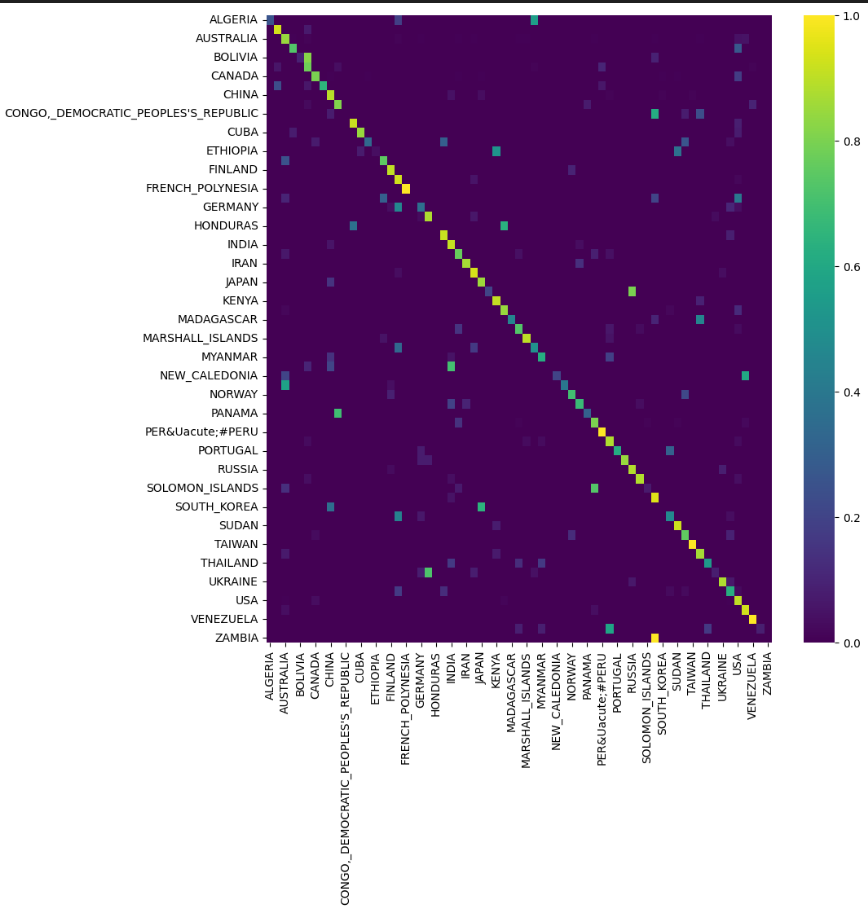
\includegraphics[width=\textwidth]{content/img/matrix-f10.png}
    \caption{Matrice de confusion pour 10 aéroports par pays minimum}
    \label{fig:matrix-f10}
\end{figure}

\begin{figure}[h!]
    \centering
    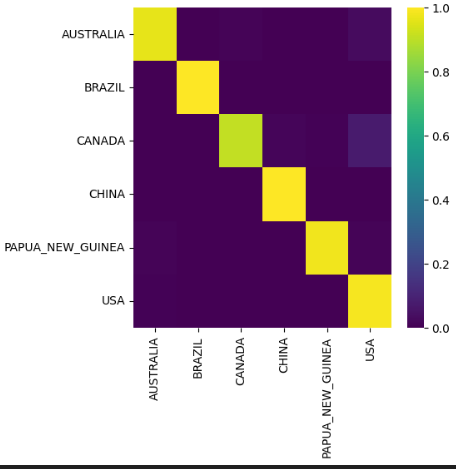
\includegraphics[width=0.3\textwidth]{content/img/matrix-f90.png}
    \caption{Matrice de confusion pour 90 aéroports par pays minimum}
    \label{fig:matrix-f90}
\end{figure}

Les résultats obtenus montrent que, globalement (il y a des exceptions), la
performance du modèle augmente à mesure que l'on diminue le nombre de pays à
classifier.\\ Cela s'explique par le fait que plus le nombre d'aéroports par
pays est faible, plus il y aura de classes différentes à prédir, et plus il y
aura de chances de tomber sur un aéroport unique au pays. Le modèle devra donc
classifier un aéroport qui n'a encore jamais été vu.\\ Cela permet donc
d'obtenir une meilleure performance du modèle.\\

La matrices (Figure \ref{fig:matrix-f10}) montre que même avec un filtrage de
10 aéroports minimum par pays, le modèle a encore du mal à classifier certains
aéroports (certains pays ont une précision de 0\%). On peut la comparer à la
matrice (Figure \ref{fig:matrix-f90}) qui montre une meilleure performance du
modèle avec un filtrage de 90 aéroports minimum par pays. On peux d'ailleurs
observer qu'il y a quelques erreurs de classification pour les pays étant
proches géographiquement.\\

La nombre d'aéroports par pays est donc un facteur important à prendre en
compte pour la classification des aéroports par pays. Des classes (pays) avec
un nombre d'aéroports trop faible à pour effet d'introduire du bruit dans les
données et de diminuer la performance du modèle.\\

\needspace{20\baselineskip}
\subsubsection{Influence des features}

Dans cette partie, j'ai testé l'influence des features sur la performance du
modèle.\\ J'ai testé les configurations suivantes : [latitude, longitude];
[latitude, longitude, population]; [population].\\ J'ai également fait varier
le nombre d'aéroports par pays pour chaque configuration de features (10, 50,
100) car il pourrait y avoir un attribut qui influence plus ou moins la
performance du modèle en fonction du nombre de classes à prédire.\\

% Table
\begin{table}[h!]
    \centering

    \begin{tabular}{|c||c|c|c|c|c|c|}
        \hline
        \textbf{Nombre d'aéroports par pays} & \multicolumn{2}{c|}{10} & \multicolumn{2}{c|}{50} & \multicolumn{2}{c|}{100}                                                          \\ \hline
        \textbf{Nombre de classes}           & \multicolumn{2}{c|}{67} & \multicolumn{2}{c|}{12} & \multicolumn{2}{c|}{4}                                                            \\ \hline \hline
        \textbf{Features}                    & \textbf{Précision}      & \textbf{Erreur}         & \textbf{Précision}       & \textbf{Erreur} & \textbf{Précision} & \textbf{Erreur} \\ \hline
        [latitude, longitude]                & 0.6407                  & 1.5146                  & 0.9266                   & 0.2872          & 0.9587             & 0.1284          \\ \hline
        [latitude, longitude, population]    & 0.6712                  & 1.6314                  & 0.9492                   & 0.2192          & 0.9835             & 0.056           \\ \hline
        [population]                         & 0.1051                  & 3.5076                  & 0.1751                   & 1.7845          & 0.7769             & 0.5597          \\ \hline

    \end{tabular}
    \caption{Influence des features sur la performance du modèle}
\end{table}

L'analyse de 'influence des features sur la performance du modèle GCN révèle
des tendances intéressantes. Globalement, l'ajout de la population aux features
de latitude et longitude améliore la précision du modèle et réduit l'erreur de
classification.\\

La combinaison des trois features - latitude, longitude et population - s'avère
la plus efficace pour la classification des pays. Ceci suggère que la
population joue un rôle significatif dans la structuration du réseau aérien et
permet au modèle de mieux discriminer les pays. Par exemple, pour 10 aéroports
par pays, la précision passe de 0.6407 à 0.6712 lorsqu'on ajoute la population
aux features de latitude et longitude.\\

Cette constatation m'a amené à explorer davantage l'influence de la population
en l'isolant des autres features. Les résultats montrent que la population
seule n'est pas suffisante pour classifier un grand nombre de pays mais quand
le nombre de classes diminue, la population devient un facteur déterminant pour
la classification. Par exemple, pour 100 aéroports par pays, la précision est
de 0.7769 avec la population seule contre. La population doit donc avoir un
impact pour créer pluste de contraste entre les différents pays. On peut donc
en déduire que la différence de population entre les USA et le Canada
(adjacents géographiquement) est une information qui a été extraite par le
modèle pour les différencier.\\

\needspace{20\baselineskip}
\subsubsection{Pondération des liens}

Après avoir examiner les features des noeuds, j'ai décidé de m'intéresser à la
pondération des liens.\\ J'ai voulu savoir si la pondération des liens pouvait
améliorer la performance du modèle.\\ J'ai testé sur différentes configurations
de nombre d'aéroports par pays (10, 50, 100) l'influence de la pondération des
liens sur la performance du modèle. Et comparé les résultats obtenus avec et
sans pondération des liens.\\

Pour pondérer les liens j'ai calculé la distance euclidienne entre les
aéroports (grâce à leurs coordonnées latitude et longitude), je l'ai normalisé
et utiliser l'inverse de cette distance comme pondération (plus les aéroports
sont proches, plus le lien est fort).\\

% Table
\begin{table}[h!]
    \centering

    \begin{tabular}{|c||c|c|c|c|c|c|}
        \hline
        \textbf{Nombre d'aéroports par pays} & \multicolumn{2}{c|}{10} & \multicolumn{2}{c|}{50} & \multicolumn{2}{c|}{100}                                                          \\ \hline \hline
        \textbf{Pondération des liens}       & \textbf{Précision}      & \textbf{Erreur}         & \textbf{Précision}       & \textbf{Erreur} & \textbf{Précision} & \textbf{Erreur} \\ \hline
        Sans pondération                     & 0.6407                  & 1.5146                  & 0.9266                   & 0.2872          & 0.9587             & 0.1284          \\ \hline
        Avec pondération                     & 0.7017                  & 1.1801                  & 0.9379                   & 0.2429          & 0.9752             & 0.0822          \\ \hline

    \end{tabular}
    \caption{Influence de la pondération des liens sur la performance du modèle}
\end{table}

Les résultats montrent que la pondération des liens améliore la performance du
modèle.\\

L'ajout de la pondération aux liens a un effet positif majeur sur la précision
du modèle et sur la réduction de l'erreur, et ce, quel que soit le nombre
d'aéroports par pays. Par exemple, pour 10 aéroports par pays, la précision
passe de 0.6407 sans pondération à 0.9379 avec pondération, tandis que l'erreur
diminue de 1.5146 à 1.1801. Cette amélioration est observée de manière
consistante pour 50 et 100 aéroports par pays.\\

Cepandant il

\needspace{20\baselineskip}
\subsubsection{Structure du graphe}

Enfin, j'ai testé les performances du modèle en faisant varier la structure du
graphe (Fully-connected, Country-based).\\ J'ai testé les performances du
modèle avec un graphe \textbf{fully-connected} et un graphe
\textbf{country-based}.\\

Cela n'a pas pour but de trouver les meilleurs hyperparamètres mais d'observer
l'influence des liens entre les noeuds sur la performance d'un modèle GCN.\\

% Table fully-connected
\begin{table}[h!]
    \centering

    \begin{tabular}{|c||c|c|c|c|c|c|}
        \hline
        \textbf{Nombre d'aéroports par pays} & \multicolumn{2}{c|}{10} & \multicolumn{2}{c|}{50} & \multicolumn{2}{c|}{100}                                                          \\ \hline \hline
        \textbf{Structure du graph}          & \textbf{Précision}      & \textbf{Erreur}         & \textbf{Précision}       & \textbf{Erreur} & \textbf{Précision} & \textbf{Erreur} \\ \hline
        Fully-connected                      & /////                   & /////                   & /////                    & /////           & 0.5537             & 1.1546          \\ \hline
        Country-based                        & 0.9928                  & 0.0826                  & 1.0                      & 0.0043          & 1.                 & 0.0011          \\ \hline
        Original                             & 0.6407                  & 1.5146                  & 0.9266                   & 0.2872          & 0.9752             & 0.0822          \\ \hline
    \end{tabular}
    \caption{Performance du modèle avec un graphe \textbf{fully-connected}} avec pondération
\end{table}

\textit{Pour des raisons de performance, j'ai testé les graphes fully-connected avec pondération uniquement pour les pays ayant un minimum de 100 aéroports}.

Le graphe "country-based", où les aéroports sont connectés uniquement aux
aéroports du même pays, offre les meilleures performances en termes de
précision et d'erreur. Il atteint une précision parfaite (1.0) pour 50 et 100
aéroports par pays minimum, avec une erreur quasi nulle. Ceci suggère que la
structure "country-based" capture efficacement les relations essentielles pour
la classification des pays.\\

Le graphe "fully-connected", où tous les aéroports sont connectés entre eux,
présente la plus faible performance, avec une précision de seulement 0.5537
pour 100 aéroports par pays. Ceci indique qu'une connectivité excessive
introduit du bruit et nuit à la capacité du modèle à discriminer les pays.\\

Ces résultats soulignent l'importance de choisir une structure de graphe
adaptée à la tâche de classification. Dans votre cas, la structure
"country-based" semble la plus pertinente car elle reflète directement les
relations géographiques et politiques qui déterminent l'appartenance d'un
aéroport à un pays mais est une structure qui peut être difficile à obtenir
dans la réalité.\\

\subsection{Mon modèle de classification}

Après avoir testé différentes configurations, j'ai choisi un modèle de
classification qui combine les éléments suivants : \\ - \textbf{Features} :
[latitude, longitude, population] \\ - \textbf{Nombre d'aéroports par pays} :
30 \\ - \textbf{Pondération des liens} : Oui \\

J'ai choisi un nombre d'aéroports par pays de 30 car il offre un bon compromis
entre le nombre de classes à prédire et la performance du modèle.\\

\begin{table}[h!]
    \centering
    \begin{tabular}{|c|c|c|c|}
        \hline
                           & \textbf{Train} & \textbf{Validation} & \textbf{Test} \\ \hline \hline
        \textbf{Précision} & 0.95           & 0.9136              & 0.8909        \\ \hline
        \textbf{Erreur}    & 0.2018         & 0.3869              & 0.5313        \\ \hline
    \end{tabular}
    \caption{Performance du modèle final}
\end{table}

Le modèle final a été entraîné sur un total de 3 153 époches, avec un taux d'apprentissage de 0.001.
Le modèle a atteint une précision d'environ 90\%.\\

La matrice de confusion (Figure \ref{fig:matrix-f30}) montre que le modèle a
une bonne capacité à discriminer les pays, avec des taux de classification
élevés pour la plupart des classes. Cependant, il y a quelques erreurs de
classification pour certains pays, en particulier pour les pays voisins ou
géographiquement proches.\\
\begin{figure}[h!]
    \centering
    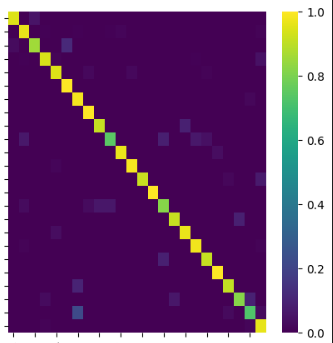
\includegraphics[width=0.4\textwidth]{content/img/final-matrix.png}
    \caption{Matrice de confusion du modèle final}
    \label{fig:matrix-f30}
\end{figure}


Nous pouvons également observer l'évolution de la précision et de l'erreur du
modèle par époque (Figures \ref{fig:acc-evol} \& \ref{fig:loss-evol}).\\

% image 
\begin{figure}[h!]
    \centering
    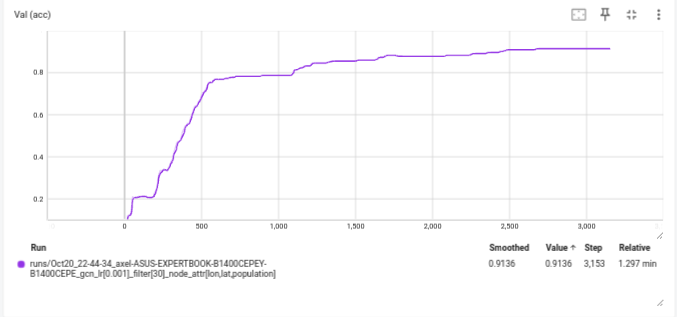
\includegraphics[width=\textwidth]{content/img/final-acc-evol.png}
    \caption{Evolution de la précision du modèle par époque}
    \label{fig:acc-evol}
\end{figure}

\begin{figure}[h!]
    \centering
    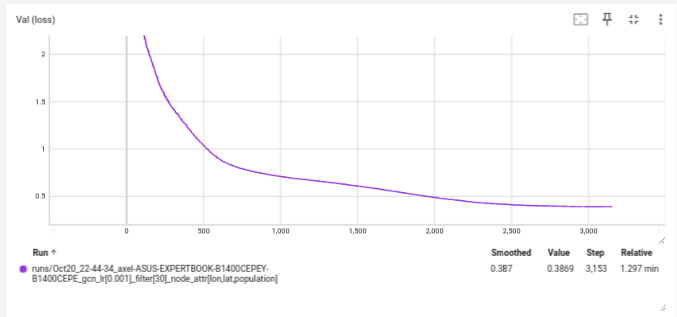
\includegraphics[width=\textwidth]{content/img/final-loss-evol.png}
    \caption{Evolution de l'erreur du modèle par époque}
    \label{fig:loss-evol}
\end{figure}


\clearpage  

\section{Conclusion}

Dans ce rapport, j'ai présenté une approche de classification des aéroports par
pays en utilisant un modèle GCN. J'ai exploré l'influence de différents facteurs
sur la performance du modèle, notamment le nombre d'aéroports par pays, les
features des noeuds, la pondération des liens et la structure du graphe.\\

J'ai constaté que le nombre d'aéroports par pays, les features des noeuds et la
pondération des liens ont un impact significatif sur la performance du modèle.
En particulier, l'ajout de la population aux features de latitude et longitude
améliore la précision du modèle, tandis que la pondération des liens renforce
les relations entre les aéroports et améliore la capacité du modèle à
discriminer les pays.\\

Enfin, j'ai identifié un modèle de classification optimal qui combine les
éléments suivants : features [latitude, longitude, population], 30 aéroports par
pays et pondération des liens. Ce modèle a atteint une précision d'environ 90\%
et est capable de prédire correctement le pays d'un aéroport dans la plupart des
cas.\\

En conclusion, cette approche de classification des aéroports par pays montre
que les modèles GCN peuvent être efficaces pour traiter des données complexes
et hétérogènes mais rencontre des limites quand le nombre de classes devient trop important.\\

Pour aller plus loin, il serait intéressant d'explorer d'autres types de modèles comme les GNNs récurrents ou les GNNs spatiaux pour améliorer la performance du modèle.

\begin{figure}[h!]
    \centering
    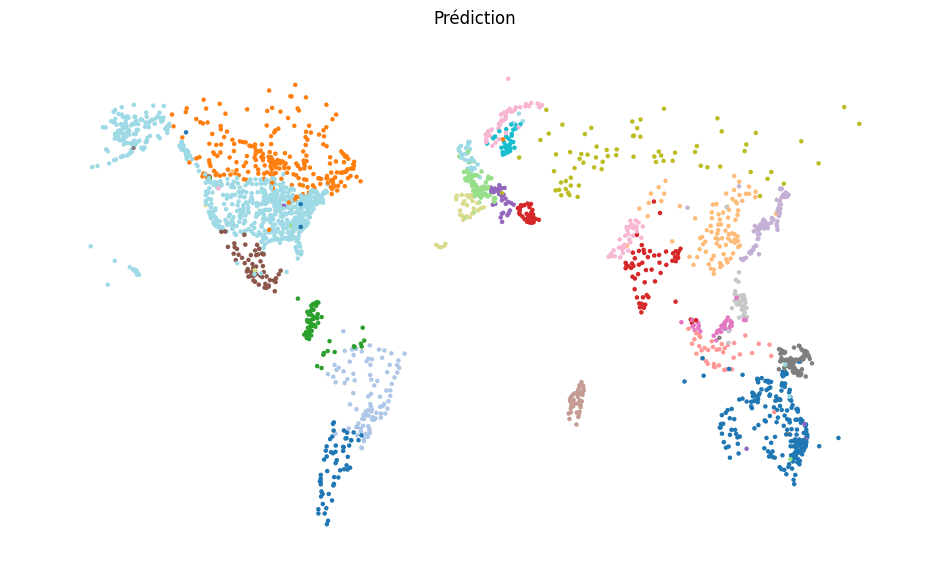
\includegraphics[width=\textwidth]{content/img/final-map.png}
    \caption{Prédictions du modèle final sur une carte}
    \label{fig:map}
\end{figure}




\end{document}